\documentclass{beamer}
\usepackage{amsfonts,amsmath,oldgerm}
\usetheme{sintef}
\usepackage{tabularx,booktabs}
\usepackage{tikz}
\usepackage[most]{tcolorbox}
\usetikzlibrary{shapes,arrows,positioning}

\newcommand{\testcolor}[1]{\colorbox{#1}{\textcolor{#1}{test}}~\texttt{#1}}

\usefonttheme[onlymath]{serif}

\titlebackground*{assets/background}

% adicionar o numero na lista final da apresentação
\setbeamertemplate{bibliography item}{\insertbiblabel}

\newcommand{\hrefcol}[2]{\textcolor{cyan}{\href{#1}{#2}}}

\title{Optimizers in deep learning}
\course{CPE 727 - Deep Learning}
\author{Ana Clara Loureiro Cruz \and Bruno Coelho Martins \and Emre Aslan \and Felipe Barreto Andrade}
\IDnumber{%
  \href{mailto:anaclaralcruz@poli.ufrj.br}{anaclaralcruz@poli.ufrj.br}\\
  \href{mailto:bruno.martins@smt.ufrj.br}{bruno.martins@smt.ufrj.br}\\
  \href{mailto:emre@gta.ufrj.br}{emre@gta.ufrj.br}\\
  \href{mailto:felipebarretoandrade@poli.ufrj.br}{felipebarretoandrade@poli.ufrj.br}
}

\begin{document}
\maketitle

\section{Introduction}

% \begin{frame}{Why Optimizers Matter}
% \begin{itemize}
%   \item \textbf{Hard landscapes:} non-convex, ill-conditioned; plateaus/saddles/sharp minima.
%   \item \textbf{Speed vs.\ stability:} momentum, adaptivity, curvature cues.
%   \item \textbf{Generalization:} optimizer choice influences minima flatness and test accuracy.
%   \item \textbf{Scaling:} large batches + mixed precision $\Rightarrow$ LARS/LAMB trust ratios.
%   \item \textbf{Anisotropy:} coordinate-wise steps (Adagrad/RMSProp/AdamW).
%   \item \textbf{Decay:} AdamW’s decoupled weight decay matters.
%   \item \textbf{Schedules:} warmup + cosine/one-cycle are often the real win.
% \end{itemize}
% \end{frame}

\begin{frame}{Donny Loves Optimization!}
\begin{center}

\includegraphics[width=0.5\textwidth]{emre_images/donkey.png}\end{center}\\Meet Donny the donkey! He’s on a mountain, trying to find the lowest valley. His adventure is like optimization in deep learning—finding the best settings for a model.
\end{frame}
\begin{frame}{What is Optimization?}\begin{itemize}
\item Donny’s goal: Walk down the mountain to the lowest point (fewest mistakes).
\item Optimization: Finding the best weights (settings) for a model to make the smallest mistakes.    
\item A loss function is like Donny’s map—it shows how far he is from the bottom.
\item The loss function measures mistakes (how wrong the model’s guesses are).  Example: Mean Squared Error (compares guesses to correct answers).
% \item Lost Function guides Donny, showing him which way to go to make fewer mistakes.  



\end{itemize}
\end{frame}
\begin{frame}{Why We Optimize?}
  \begin{figure}
    \centering
    \includegraphics[width=0.4\textwidth]{emre_images/localminima.png}
  \end{figure}
  \begin{itemize}
    \item \textbf{Goal}: Find settings (weights) that make the \textit{fewest mistakes} for accurate predictions.
    \item Ensures the model works great on \textit{new, unseen data} (generalization).
    \item The map is tricky---wrong dips and flat spots can slow us down, but we aim for the \textit{best spot}!
  \end{itemize}
\end{frame}
\section{Gradient Descent}
\begin{frame}{What exactly is a gradient?}
\begin{itemize}
  \item \text Gradient is just a bunch of partial derivatives. This means that if we have some function of multiple variables, its gradient is just a vector of the function’s derivatives with respect to each of its variables.
  \item \text The gradient has a fascinating property: it points in the direction where the function grows fastest! Correspondingly, the opposite direction is where the function decreases fastest!
  \item \text Since our goal is to minimize the loss function, the best course of action is to take a “step” in the direction where the function decreases fastest, which, as we saw, is the direction opposite to where the gradient points. \cite{lu2024gradientdescentstochasticoptimization}
  
\end{itemize}
\end{frame}
\begin{frame}{Gradient Descent (GD) Optimization}
Donny the donkey navigates the loss landscape by taking steps opposite the steepest slope! The update rule for model parameters is:
\[
\theta_{t+1} = \theta_t - \eta \nabla_{\theta} J(\theta_t)
\]
Where:
\begin{itemize}
    \item $\theta_t$: Model parameters at iteration $t$ (e.g., weights).
    \item $\eta$: Learning rate (step size for Donny’s moves).
    \item $\nabla_{\theta} J(\theta_t)$: Gradient of the loss function, computed over the entire dataset, pointing to the steepest increase.
    \item $\theta_{t+1}$: Updated parameters after each epoch (full pass over data). \cite{chandra2022gradientdescentultimateoptimizer}
\end{itemize}
\end{frame}
% \begin{frame}{Gradient Descent (GD) Optimization}
% Using the Gradient Decent optimization algorithm, the weights are updated incrementally after each epoch (= pass over the training dataset).

% The magnitude and direction of the weight update is computed by taking a step in the opposite direction of the cost gradient. \cite{chandra2022gradientdescentultimateoptimizer} \\
% \begin{equation}
% \Delta w_j = -\eta \frac{\partial J}{\partial w_j},
% \end{equation} \\
% where $\eta$  is the learning rate. The weights are then updated after each epoch via the following update rule: \\
% \begin{equation}
% w := w + \Delta w,
% \end{equation}

% \end{frame}

% \begin{frame}{}
% where $\Delta w$ is a vector containing the weight updates for each weight coefficient $w$. These are computed as follows: \\
% \begin{equation}
% \Delta w_j = -\eta \frac{\partial J}{\partial w_j},
% \end{equation} \\
% \begin{align}
% \Delta w_j &= -\eta \frac{\partial J}{\partial w_j} = -\eta \sum_i \left( \text{target}^{(i)} - \text{output}^{(i)} \right) \left( -x_j^{(i)} \right) \\
% &= \eta \sum_i \left( \text{target}^{(i)} - \text{output}^{(i)} \right) x_j^{(i)}.
% \end{align}
% \end{frame}
\begin{frame}{}
\begin{itemize}
    \item Gradient Descent updates weights by moving opposite the gradient of the cost function to reach the minimum.
    \item Each step’s size is determined by the learning rate.\cite{bottou1998online}
\end{itemize} 

\centering
\includegraphics[width=0.5\textwidth]{emre_images/gd_line_search.png}
\end{frame}

\begin{frame}{Scaling Gradient Descent}\begin{itemize}
% “SGD is the workhorse of machine learning.” — Yoshua Bengio
\item Gradient Descent Challenge: Computing gradients on all data is computationally expensive, especially for large neural network datasets.
\item Stochastic Gradient Descent (SGD): Updates weights using one data point, taking steps based on an estimated steepest descent, ideal for big datasets.\cite{ruder2017overviewgradientdescentoptimization}
\includegraphics[width=0.7\textwidth]{emre_images/stoch_comp.png}
\end{itemize}
\end{frame}
\begin{frame}{Scaling Gradient Descent}
\begin{itemize}
\item SGD’s Strength: By the law of large numbers, single-data-point gradients average close to the true gradient, despite some zigzagging. \cite{erd1970new}
\item Minibatch Gradient Descent: Uses a small batch of examples for gradient computation, balancing speed and accuracy as a middle ground. \cite{khirirat2017mini}
\end{itemize}

    \includegraphics[width=0.95\textwidth]{emre_images/big3.png}


\end{frame}
\begin{frame}{Stochastic Gradient Descent (SGD) Formulation}
Given a loss function $L(\theta, x_i, y_i)$ for a model with parameters $\theta$, a single data point $(x_i, y_i)$, and a learning rate $\eta$, the SGD update rule for the parameters at iteration $t$ is:
\[
\theta_{t+1} = \theta_t - \eta \nabla_{\theta} L(\theta_t, x_i, y_i)
\]
Where:
\begin{itemize}
    \item $\theta_t$: Model parameters at iteration $t$.
    \item $\eta$: Learning rate (step size).
    \item $\nabla_{\theta} L(\theta_t, x_i, y_i)$: Gradient of the loss function with respect to $\theta$, computed using a single randomly selected data point $(x_i, y_i)$.
    \item $\theta_{t+1}$: Updated parameters after the step. \cite{bottou1998online}
\end{itemize}
\end{frame}
\begin{frame}{Why Stochastic Gradient Descent (SGD)?}
\begin{itemize}
    \item \textbf{Large Datasets}: SGD updates parameters using single data points, making it faster and more efficient than traditional gradient descent for massive datasets.\cite{bottou2010large}
    \item \textbf{Non-Convex Problems}: SGD’s random updates help escape local minima, increasing the chance of finding the global minimum in non-convex optimization. \cite{lei2019stochastic}
    \item \textbf{Online Learning}: SGD supports real-time updates with new data, ideal for applications where data arrives continuously.\cite{jothimurugesan2018variance}
\end{itemize}
\end{frame}

% \begin{frame}{Intuition in Two Pictures}
% \begin{columns}[T,onlytextwidth]
% \begin{column}{0.48\textwidth}
% \centering
% \textbf{Sharp vs.\ Flat Minima}\\[0.3em]
% \begin{tikzpicture}[scale=0.9]
%   \draw[->] (-2.2,0) -- (2.2,0) node[right] {$\theta$};
%   \draw[->] (0,-0.3) -- (0,2.8) node[above] {$\mathcal{L}$};
%   % flat well
%   \draw[thick,blue] plot[smooth] coordinates {(-2,2) (-1.4,1.2) (-0.8,0.8) (-0.2,0.7) (0.4,0.8) (1.0,1.2) (1.6,2)};
%   % sharp well
%   \draw[thick,red] plot[smooth] coordinates {(-2,2.3) (-1.2,1.4) (-0.4,0.3) (0,0.1) (0.4,0.3) (1.2,1.5) (2,2.4)};
%   \node[blue] at (-0.4,0.4) {flat};
%   \node[red]  at (0.8,0.6)  {sharp};
% \end{tikzpicture}

% {\small SAM/SGD tend to favor flatter minima $\Rightarrow$ better test performance.}
% \end{column}
% \begin{column}{0.48\textwidth}
% \centering
% \textbf{Paths on an Anisotropic Bowl}\\[0.3em]
% \begin{tikzpicture}[scale=0.9]
%   % axes
%   \draw[->] (-2.2,0) -- (2.2,0) node[right] {$\theta_1$};
%   \draw[->] (0,-2.2) -- (0,2.2) node[above] {$\theta_2$};
%   % contours (ellipses)
%   \foreach \r in {0.6,1.0,1.4,1.8} {
%     \draw[gray!60] (0,0) ellipse ({2*\r} and {0.8*\r});
%   }
%   % SGD path
%   \draw[thick,orange,-stealth] (-1.8,1.6) .. controls (-1.5,1.0) .. (-1.2,0.6)
%                                 .. controls (-0.9,0.3) .. (-0.6,0.15) .. controls (-0.3,0.08) .. (-0.15,0.04);
%   \node[orange] at (-1.5,1.5) {SGD};
%   % AdamW path
%   \draw[thick,blue,-stealth] (-1.8,1.6) .. controls (-1.0,1.0) .. (-0.5,0.5)
%                              .. controls (-0.25,0.25) .. (-0.05,0.05);
%   \node[blue] at (-0.9,0.9) {AdamW};
% \end{tikzpicture}

% {\small AdamW adapts steps per-coordinate; momentum smooths zig-zagging.}
% \end{column}
% \end{columns}
% \end{frame}

% \begin{frame}{Common notation}
% Objective:  \min_\theta f(\theta)

% Stochastic gradient at step t: g_t = \nabla_\theta f_t(\theta_t)

% Base LR: \eta_t; small \varepsilon > 0 for numerical stability.
% \end{frame}


% \section{Plain First-Order}

% \begin{frame}{SGD (baseline) \cite{gradientDescent}}
% \[
%   \theta_{t+1} = \theta_t - \eta_t\, g_t
% \]
% \begin{itemize}
%   \item Sets the stage for momentum, adaptivity, and curvature.
%   \item Sensitive to scale/conditioning; zig-zags in anisotropic valleys.
% \end{itemize}
% \textbf{Example:} \emph{SGD (vanilla)}
% \end{frame}

\section{Momentum Variants}

% \begin{frame}{Polyak \& Nesterov}
% \textbf{Polyak Momentum (EMA of gradients):}
% \[
%   v_t = \beta\, v_{t-1} + (1-\beta)\, g_t,\qquad
%   \theta_{t+1} = \theta_t - \eta_t\, v_t
% \]
% \textbf{Nesterov Momentum (look-ahead):}
% \[
%   \tilde{\theta}_t = \theta_t - \eta_t \beta v_{t-1},\quad
%   v_t = \beta v_{t-1} + g(\tilde{\theta}_t),\quad
%   \theta_{t+1} = \theta_t - \eta_t v_t
% \]

% \textbf{Example:} \emph{SGD + Momentum, Nesterov}
% \end{frame}

\begin{frame}{From SGD to Momentum: Why We Need It}
\begin{itemize}
  \item In standard Gradient Descent or SGD, parameters are updated by:
  \[
    \theta_{t+1} = \theta_t - \eta\, g_t
  \]
  \item Where:
  \begin{itemize}
    \item $\theta_t$: model parameters at iteration $t$
    \item $g_t = \nabla_\theta f_t(\theta_t)$: gradient of the loss
    \item $\eta$: learning rate (step size)
  \end{itemize}
  \item This simple rule moves directly opposite to the gradient.
  \item \textbf{Problem:} In narrow or curved valleys, the gradient direction changes quickly, causing \textbf{zig-zag motion}.
  \item We need a way to \textbf{smooth} these updates and keep consistent direction across steps.
\end{itemize}
\end{frame}

\begin{frame}{Momentum: Adding Memory to SGD}
\textbf{Idea:} Add “inertia”, accumulate a moving average of past gradients:
\[
  v_t = \beta v_{t-1} + (1-\beta) g_t, \qquad
  \theta_{t+1} = \theta_t - \eta v_t
\]

\textbf{Where:}
\begin{itemize}
  \item $v_t$: velocity (smoothed gradient direction)
  \item $\beta$: momentum coefficient (typically $0.9$)
  \item $\eta$: learning rate
\end{itemize}

\textbf{Effect:}
\begin{itemize}
  \item Reduces oscillations across steep axes.
  \item Accelerates along consistent descent directions.
  \item Leads to faster and more stable convergence.
\end{itemize}

\textbf{Visualization:} Like rolling a ball downhill — it gains speed in the main slope direction and ignores small bumps.
\end{frame}






\section{Adaptive First-Order}

% \begin{frame}{Per-Coordinate Step Sizes}
% \textbf{Adagrad (cumulative second moment):}
% \[
%   s_t = s_{t-1} + g_t \odot g_t,\qquad
%   \theta_{t+1} = \theta_t - \frac{\eta}{\sqrt{s_t} + \varepsilon}\odot g_t
% \]
% \textbf{RMSProp (exponential second moment):}
% \[
%   s_t = \rho s_{t-1} + (1-\rho)\, g_t \odot g_t,\qquad
%   \theta_{t+1} = \theta_t - \frac{\eta}{\sqrt{s_t} + \varepsilon}\odot g_t
% \]
% \end{frame}

\begin{frame}{Adaptive Learning Rates: Intuition (Adagrad vs. RMSProp)}
\begin{itemize}
  \item \textbf{Motivation:} Different parameters experience very different gradient magnitudes.
  \item \textbf{Adagrad:}
    \begin{itemize}
      \item Accumulates the sum of squared gradients $\Rightarrow$ per-parameter step sizes shrink over time.
      \item \textbf{Pros:} Excellent for sparse features.
      \item \textbf{Cons:} Accumulator grows without bound $\Rightarrow$ steps can “die”.
    \end{itemize}
  \item \textbf{RMSProp:}
    \begin{itemize}
      \item Uses an \emph{exponential moving average} of squared gradients $\Rightarrow$ finite memory of the past.
      \item \textbf{Pros:} Stabilizes step scale throughout training.
      \item \textbf{Cons:} Sensitive to the EMA coefficient $\rho$.
    \end{itemize}
  \item \textbf{Bridge to Adam:} Combine momentum (first moment) + RMSProp-like scaling (second moment) + bias correction.
\end{itemize}

\vspace{0.4em}
\end{frame}


\begin{frame}{Adam: Motivation and Intuition}
\begin{itemize}
  \item Adaptive Moment Estimation was proposed in 2014 by Kingma and Ba .
  \item Combines \textbf{momentum} (smooths noisy gradients) with \textbf{adaptive learning rates} (per-parameter step scaling).
  \item Inspired by ideas from \emph{RMSProp} (adaptive second moment) and \emph{Momentum} (EMA of gradients).
  \item Works well out-of-the-box; minimal tuning, fast convergence.
  \item Default optimizer for many architectures: CNNs, Transformers, LLMs.
\end{itemize}
\end{frame}

\begin{frame}{Adam: Adaptive Moment Estimation}
\textbf{Formal equations:}
\[
  m_t = \beta_1 m_{t-1} + (1 - \beta_1) g_t, \qquad
  v_t = \beta_2 v_{t-1} + (1 - \beta_2) g_t \odot g_t
\]
\[
  \hat{m}_t = \frac{m_t}{1 - \beta_1^t}, \qquad
  \hat{v}_t = \frac{v_t}{1 - \beta_2^t}, \qquad
  \theta_{t+1} = \theta_t - \eta \frac{\hat{m}_t}{\sqrt{\hat{v}_t} + \varepsilon}
\]

\vspace{0.35em}
\textbf{Where:}
{\footnotesize
\begin{itemize}
  \item $\theta_t$: model parameters at iteration $t$; $\varepsilon$: small constant for numerical stability ($10^{-8}$).
  \item $m_t$: first moment (EMA of gradients); $\beta_1$: decay factor for the mean (≈ 0.9).
  \item $v_t$: second moment (EMA of squared gradients); $\beta_2$: decay factor for variance (≈ 0.999).
  \item $\hat{m}_t,\ \hat{v}_t$: bias-corrected versions to remove initialization bias.
  \item $\odot$: element-wise multiplication (Hadamard product).
\end{itemize}
}

\vspace{0.35em}
{\footnotesize
Introduced in \textbf{Adam}~\cite{kingma2014adam}. Combines momentum (first moment) and adaptive scaling (second moment).  
Common variants: AMSGrad~\cite{reddi2019amsgrad}, RAdam~\cite{liu2019radam}.
}
\end{frame}

\begin{frame}{AdamW: Decoupled Weight Decay}
\textbf{Update rule:}
\[
  \theta_{t+1} = (1 - \eta \lambda)\,\theta_t - \eta \frac{\hat{m}_t}{\sqrt{\hat{v}_t} + \varepsilon}
\]

\vspace{0.35em}
\textbf{Key idea:}
\begin{itemize}
  \item In the original Adam, weight decay (L2 regularization) was included \emph{inside} the adaptive term, interfering with per-parameter learning rates.
  \item AdamW \textbf{decouples} weight decay from the gradient-based update.
  \item This preserves clean regularization and improves generalization, especially in large models (Transformers, ViTs).
\end{itemize}

\vspace{0.35em}
\textbf{Where:}
{\footnotesize
\begin{itemize}
  \item $\lambda$: weight decay coefficient. $(1 - \eta \lambda)$ applies pure L2 regularization.
\end{itemize}
}

\vspace{0.35em}
{\footnotesize
Proposed in \textbf{AdamW}~\cite{loshchilov2017decoupled}.  
Later analyses on convergence and decay scaling:  
\cite{ding2023adamfamily,wang2024adamwdecay}.
}
\end{frame}




\begin{frame}{Adam: Step-by-Step}
\begin{enumerate}
  \item Compute gradient $g_t = \nabla_\theta f_t(\theta_t)$.
  \item Update first moment (mean): $m_t = \beta_1 m_{t-1} + (1-\beta_1) g_t$.
  \item Update second moment (variance): $v_t = \beta_2 v_{t-1} + (1-\beta_2) g_t^2$.
  \item Bias-correct: $\hat{m}_t = m_t / (1-\beta_1^t)$, $\hat{v}_t = v_t / (1-\beta_2^t)$.
  \item Parameter update:
  \[
    \theta_{t+1} = \theta_t - \eta \frac{\hat{m}_t}{\sqrt{\hat{v}_t} + \varepsilon}
  \]
\end{enumerate}
{\small Typical defaults: $\beta_1 = 0.9,\ \beta_2 = 0.999,\ \varepsilon = 10^{-8}$}

{\footnotesize
Algorithm details follow \cite{kingma2014adam}; bias corrections mitigate initialization effects in early iterations.
}

\end{frame}


% Requires: \usepackage{tikz}
% (You already used TikZ earlier, so this should compile as-is.)

\begin{frame}{Adam: Geometric Interpretation}
\begin{columns}[T,onlytextwidth]
\begin{column}{0.52\textwidth}
\begin{itemize}
  \item \textbf{Anisotropy:} curvature differs across coordinates.
  \item \textbf{SGD (momentum):} faster than vanilla SGD, but still zig-zags along the steep axis.
  \item \textbf{Adam/AdamW:} per-parameter scaling (via $\sqrt{\hat v_t}$) damps steps where gradients are large and allows larger steps where they are small.
  \item \textbf{Effect:} straighter trajectory toward the minimum, fewer oscillations.
\end{itemize}
\end{column}
\begin{column}{0.46\textwidth}
\centering
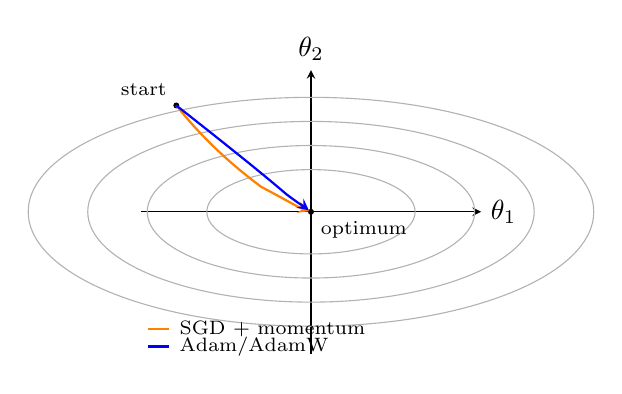
\begin{tikzpicture}[scale=0.9,>=stealth]
  % Axes
  \draw[->] (-2.4,0) -- (2.4,0) node[right] {$\theta_1$};
  \draw[->] (0,-2.0) -- (0,2.0) node[above] {$\theta_2$};

  % Anisotropic level sets (ellipses)
  \foreach \r in {0.7,1.1,1.5,1.9} {
    \draw[gray!60] (0,0) ellipse ({2.1*\r} and {0.85*\r});
  }

  % Start and optimum
  \fill[black] (-1.9,1.5) circle (1.2pt) node[above left] {\scriptsize start};
  \fill[black] (0,0) circle (1.2pt) node[below right] {\scriptsize optimum};

  % SGD+Momentum path (zig-zag)
  \draw[thick,orange,-stealth]
    (-1.9,1.5)
    .. controls (-1.5,1.0) and (-1.1,0.65) ..
    (-0.7,0.35)
    .. controls (-0.45,0.22) and (-0.28,0.12) ..
    (-0.16,0.06)
    .. controls (-0.09,0.04) and (-0.05,0.02) ..
    (-0.02,0.01);

  % Adam/AdamW path (straighter)
  \draw[thick,blue,-stealth]
    (-1.9,1.5)
    .. controls (-1.2,0.95) and (-0.7,0.55) ..
    (-0.35,0.25)
    .. controls (-0.18,0.12) and (-0.08,0.06) ..
    (-0.03,0.02);

  % Legend
  \draw[orange,thick] (-2.3,-1.65) -- (-2.0,-1.65) node[right,black] {\scriptsize SGD + momentum};
  \draw[blue,thick]   (-2.3,-1.9)  -- (-2.0,-1.9)  node[right,black] {\scriptsize Adam/AdamW};
\end{tikzpicture}
\end{column}
\end{columns}

\vspace{0.5em}
{\footnotesize Adam rescales each coordinate by $\frac{1}{\sqrt{\hat v_t}+\varepsilon}$, so directions with persistently large gradients get smaller steps, reducing oscillations across the high-curvature axis and yielding a more direct path.}
\end{frame}

\begin{frame}{Practical Notes on Adam}
\begin{itemize}
  \item Default LR often $1\text{e-3}$ for small models; $3\text{e-4}$ for large ones.
  \item Combine with learning rate schedules (warmup + cosine decay).
  \item Works well with mixed-precision (FP16/BF16) training.
  \item Common in NLP/ViTs; sometimes replaced by SGD for vision due to generalization.
  \item Always prefer \textbf{AdamW} over Adam (decoupled weight decay).
\end{itemize}

{\footnotesize
Recent analyses such as \cite{ding2023adamfamily,wang2024adamwdecay} revisit weight decay scaling for modern large-scale training.
}

\end{frame}




\section{Learning-rate (LR) Schedulers}

\begin{frame}{Why use an LR scheduler?}
\begin{itemize}
  \item Schedulers dynamically change the learning rate during training to improve convergence and generalization.
  \item They can warm up, decay, oscillate, or respond to validation performance.
  \item Choosing the right scheduler depends on model size, batch size, dataset, and training stability.
\end{itemize}

{\footnotesize
 \cite{pytorchdocs}
}
\end{frame}

\begin{frame}{LambdaLR — Flexible functional schedules}
\textbf{What it does:} Applies a user-defined function that scales the base learning rate for each epoch or step.

\textbf{When to use:}
\begin{itemize}
  \item When you need a fully customized learning rate function.
  \item Useful in research or experiments that require nonstandard decay shapes.
\end{itemize}
\end{frame}

\begin{frame}{MultiplicativeLR — repeated multiplicative updates}
\textbf{What it does:} Multiplies the current learning rate by a specified factor each iteration.

\textbf{When to use:}
\begin{itemize}
  \item When you want a simple multiplicative decay or growth pattern.
  \item Ideal for smooth scaling without abrupt changes.
\end{itemize}
\end{frame}

\begin{frame}{StepLR \& MultiStepLR — discrete drops}
\textbf{What they do:} StepLR reduces the learning rate by a fixed factor every few epochs. MultiStepLR applies drops at specific milestone epochs.

\textbf{When to use:}
\begin{itemize}
  \item When you have prior knowledge about when to slow down learning.
  \item Suitable for traditional deep learning setups like ResNet training.
  \item StepLR for regular intervals; MultiStepLR for manually chosen epochs.
\end{itemize}
\end{frame}

\begin{frame}{ConstantLR \& LinearLR}
\textbf{What they do:} ConstantLR maintains a fixed multiplier for a few iterations. LinearLR gradually increases or decreases the rate linearly between two factors.

\textbf{When to use:}
\begin{itemize}
  \item Ideal for warmup phases before the main schedule begins.
  \item LinearLR provides a smooth transition from a small to a normal learning rate.
\end{itemize}
\end{frame}

\begin{frame}{ExponentialLR \& PolynomialLR}
\textbf{What they do:} ExponentialLR decays the learning rate exponentially over epochs. PolynomialLR uses a polynomial decay curve.

\textbf{When to use:}
\begin{itemize}
  \item ExponentialLR for steady and continuous decay over long training runs.
  \item PolynomialLR when you want slower decay near the end of training or more control over the tail behavior.
\end{itemize}
\end{frame}

\begin{frame}{CosineAnnealingLR — smooth annealing}
\textbf{What it does:} Follows a cosine-shaped curve from a maximum to a minimum learning rate.

\[
\eta_{t+1} = \eta_{\min} + (\eta_t - \eta_{\min}) \cdot 
\frac{1 + \cos\left( \frac{T_{\text{cur}}}{T_{\max}} \pi \right)}
{1 + \cos\left( \frac{T_{\text{cur}} + 1}{T_{\max}} \pi \right)}
\]

\smallskip
\textbf{Where:}
\begin{itemize}
  \item $\eta_t$ — learning rate at step $t$
  \item $T_{\text{cur}}$ — number of epochs since the last restart
  \item $T_{\max}$ — maximum number of epochs in a cycle
\end{itemize}

\textbf{When to use:}
\begin{itemize}
  \item Recommended for long training sessions where smooth convergence is desired.
  \item Commonly paired with warmup for large-scale models.
  \item Provides a graceful reduction toward the end of training.
\end{itemize}
\end{frame}

\begin{frame}{ChainedScheduler \& SequentialLR — combining schedules}
\textbf{What they do:} ChainedScheduler applies multiple schedulers together; SequentialLR runs them in sequence over predefined intervals.

\textbf{When to use:}
\begin{itemize}
  \item When combining warmup, decay, or cyclic phases.
  \item SequentialLR is ideal for warmup followed by a main schedule.
  \item ChainedScheduler is used for composite effects applied at the same time.
\end{itemize}
\end{frame}

\begin{frame}{ReduceLROnPlateau — metric-driven reduction}
\textbf{What it does:} Reduces the learning rate when a monitored validation metric stops improving.

\textbf{When to use:}
\begin{itemize}
  \item When model performance does not improve consistently.
  \item Common in fine-tuning or transfer learning scenarios.
  \item Useful when the ideal decay timing is unknown.
\end{itemize}
\end{frame}

\begin{frame}{CyclicLR — cyclical policies}
\textbf{What it does:} Cycles the learning rate between a minimum and maximum value, forming a triangular or exponential pattern.

\textbf{When to use:}
\begin{itemize}
  \item When you want the optimizer to periodically explore new minima.
  \item Suitable for smaller models and datasets with high gradient noise.
  \item Encourages faster convergence and can escape plateaus.
\end{itemize}
\end{frame}

\begin{frame}{OneCycleLR — single-cycle super-convergence}
\textbf{What it does:} Increases the learning rate from a small value to a peak and then decreases it to near zero in one cycle.

\textbf{When to use:}
\begin{itemize}
  \item When aiming for very fast convergence (super-convergence).
  \item Works well for vision and classification tasks with per-batch updates.
  \item Best used when the total number of iterations is known beforehand.
\end{itemize}
\end{frame}

\begin{frame}{Practical recommendations (summary)}
\begin{itemize}
  \item \textbf{Warmup:} LinearLR or ConstantLR at the start of training.
  \item \textbf{Stable defaults:} StepLR or MultiStepLR for traditional pipelines.
  \item \textbf{Modern default:} Warmup followed by CosineAnnealingLR.
  \item \textbf{Fast training:} OneCycleLR or CyclicLR for rapid convergence.
  \item \textbf{Dynamic control:} ReduceLROnPlateau when validation loss drives the schedule.
  \item \textbf{Composition:} SequentialLR or ChainedScheduler for complex setups.
\end{itemize}
\end{frame}

\section{Beyond First Order}

\begin{frame}{First vs Second Derivative (1D intuition)}
\small
\begin{columns}[T,onlytextwidth]
\begin{column}{0.55\textwidth}
\begin{itemize}\itemsep0.35em
  \item The \textbf{first derivative} $f'(x)$ gives the \emph{slope} (direction of change).
  \item The \textbf{second derivative} $f''(x)$ gives the \emph{curvature} (how the slope bends).
  \item Where $f'(x)=0$:
  \begin{itemize}
     \item $f''(x)>0$ → local minimum (curve opens upward)
     \item $f''(x)<0$ → local maximum (curve opens downward)
  \end{itemize}
  \item For many dimensions:
    \begin{itemize}
     \item $f'(x)$ → $\nabla f(\theta)$
     \item $f''(x)$ → $H = \nabla^2 f(\theta)$
  \end{itemize}
\end{itemize}

\end{column}

\begin{column}{0.45\textwidth}
\centering
\begin{tikzpicture}[scale=0.95,>=stealth]
  % axes
  \draw[->] (-3.1,0) -- (3.3,0) node[right] {$x$};
  \draw[->] (0,-0.6) -- (0,2.8) node[above] {$f(x)$};

  % curve
  \draw[thick,blue!70!black,domain=-2.6:2.6,samples=80]
       plot(\x,{0.2*\x*\x + 0.5*sin(\x r) + 1.0});

  % tangent at -2,0,2
  \foreach \x/\col in { 0/green!60!black}{
     \pgfmathsetmacro{\y}{0.2*\x*\x + 0.5*sin(\x) + 1.0}
     \pgfmathsetmacro{\slope}{0.4*\x + 0.5*cos(\x)}
     \draw[thick,\col] (\x-0.8,{\y-0.8*\slope}) -- (\x+0.8,{\y+0.8*\slope});
     \filldraw[black] (\x,\y) circle(1pt);
  }
  \node[align=center,font=\scriptsize,green!60!black] at (0.6,0.6)
       {\\$f'(x)>0$\\$f''(x)>0$};
\end{tikzpicture}
{\footnotesize
\cite{goodfellow2016deep}
}
\end{column}
\end{columns}
\end{frame}

\begin{frame}{Why going beyond first order?}
\small
\begin{itemize}
  \item First-order methods (SGD, Adam, etc.) rely only on the gradient $\nabla f(\theta)$.
  \item Second-order methods also use curvature information, via the Hessian $H = \nabla^2 f(\theta)$.
  \item They adapt the step direction and magnitude according to local curvature:
  \[
     \theta_{t+1} = \theta_t - H_t^{-1} \nabla f(\theta_t)
  \]
  \item This can greatly accelerate convergence near the optimum (quadratic rate).
\end{itemize}

{\footnotesize
\cite{goodfellow2016deep, boyd2004convex}.
}
\end{frame}


\begin{frame}{Newton’s Method in ML}
\small

Starting from a second-order Taylor expansion around the current point $\theta_t$:
\[
f(\theta_t + \Delta) \approx 
f(\theta_t)
+ \nabla f(\theta_t)^\top \Delta
+ \tfrac{1}{2} \Delta^\top H_t \Delta
\]

\vspace{6pt}
\begin{itemize}
  \item The \textbf{gradient} $\nabla f(\theta_t)$ gives the local slope (first-order info).
  \item The \textbf{Hessian} $H_t$ gives the local curvature (second-order info).
  \item Minimizing this local quadratic model leads to:
  \[
  H_t \Delta_t = -\nabla f(\theta_t)
  \quad \Rightarrow \quad
  \theta_{t+1} = \theta_t + \Delta_t
  \]
\end{itemize}

\vspace{6pt}
\textbf{Interpretation:}
Instead of taking small steps like gradient descent,
Newton’s Method uses curvature to \textbf{jump directly to the minimum}
of the local parabola approximation.

\end{frame}

\begin{frame}{Newton’s Method in ML \cite{boyd2004convex}}
\small
\begin{columns}[T,totalwidth=\textwidth]
\begin{column}{0.56\textwidth}
\textbf{Algorithm:}
\[
H_t \Delta_t = -\nabla f(\theta_t), \qquad \theta_{t+1} = \theta_t + \Delta_t
\]

\textbf{Characteristics:}
\begin{itemize}
  \item Converges in few iterations for convex, well-conditioned problems.
  \item Requires Hessian computation or its inverse.
\end{itemize}

\textbf{Applications:}
\begin{itemize}
  \item Generalized Linear Models (as Iteratively Reweighted Least Squares).
  \item Gaussian process optimization, small neural nets, or fine-tuning.
\end{itemize}
\end{column}
\begin{column}{0.44\textwidth}
\centering
\begin{figure}
  \includegraphics[width=\linewidth]{emre_images/newton.png}
  \caption{\footnotesize Visual representation of Newton algorithm in 1D \cite{newton-imagem}.}
\end{figure}
\end{column}
\end{columns}
\end{frame}

\begin{frame}{BFGS \cite{goodfellow2016deep}}
\small
\textbf{Idea:} Approximate the inverse Hessian $B_t \approx H_t^{-1}$ using only gradients and parameter steps.

\textbf{Secant condition:}
\[
B_{t+1} y_t = s_t, \quad 
s_t = \theta_{t+1} - \theta_t, \quad
y_t = \nabla f(\theta_{t+1}) - \nabla f(\theta_t)
\]

\textbf{BFGS update:}
\[
B_{t+1} =
B_t + 
\frac{(s_t^\top y_t + y_t^\top B_t y_t)(s_t s_t^\top)}{(s_t^\top y_t)^2}
- \frac{B_t y_t s_t^\top + s_t y_t^\top B_t}{s_t^\top y_t}
\]

\textbf{Properties:}
\begin{itemize}
  \item Curvature-aware steps without computing $H_t$.
  \item Converges superlinearly for smooth convex functions.
\end{itemize}

\textbf{Limitations:}
\begin{itemize}
  \item Requires storing full $B_t \in \mathbb{R}^{d\times d}$ → $O(d^2)$ memory.
  \item Sensitive to noisy gradients and non-convexity.
\end{itemize}
\end{frame}


\begin{frame}{Limited BFGS \cite{lbfgs}}
\small
\textbf{Idea:} Keeping only the last $m$ correction pairs $(s_i, y_i)$ to build $B_t^{-1}$ implicitly.

\textbf{Two-loop recursion:}
\begin{enumerate}\itemsep0.2em
  \item Compute $\alpha_i = \rho_i\, s_i^\top q$, where $\rho_i = 1/(y_i^\top s_i)$.
  \item Recursively apply curvature corrections backward, then forward:
  \[
  p_t = -H_t \nabla f_t \approx -\hat{B}_t \nabla f_t
  \]
  (without storing full $B_t$).
\end{enumerate}

\textbf{Application:}
\begin{itemize}
  \item Classical ML and small neural net fine-tuning.
\end{itemize}

\textbf{Limitations:}
\begin{itemize}
  \item Still needs line search; not suited to noisy minibatches.
  \item Slower wall-time per iteration than SGD/Adam for large-scale deep nets.
\end{itemize}

\end{frame}


\begin{frame}{Modern Successors: Curvature Approximations}
\small

\begin{itemize}
  \item \textbf{Hessian-Free Optimization} \cite{martens2010deep}: uses matrix-vector products $Hv$ without forming $H$.
  \item \textbf{K-FAC} \cite{ba2017distributed}: Kronecker-factored preconditioning for layerwise curvature.
  \item \textbf{Shampoo} \cite{gupta2018shampoo}: factored 2nd-order preconditioners for large tensors.
\end{itemize}

\end{frame}



\section{Summary}
\newtcolorbox{opcard}[1]{colback=gray!5,colframe=gray!40,arc=2mm,boxrule=.5pt,title=\textbf{#1}}

\begin{frame}{Optimizer comparison}
\footnotesize
\begin{columns}[t]
\begin{column}{.5\textwidth}
\begin{opcard}{SGD + Momentum (Polyak/Nesterov)}
\textbf{Behaviour:} low memory.\par
\textbf{Cons:} sensible to LR.\par
\textbf{Use:} CNN/vision with cosine+warmup.
\end{opcard}

\begin{opcard}{Adam / AdamW}
\textbf{Behaviour:} momentum + adaptative; fast.\par
\textbf{Cons:} can generalize worst than SGD.\par
\textbf{Use:} Transformers/ViTs/LLMs, mixed precision.
\end{opcard}
\end{column}
\begin{column}{.5\textwidth}
\begin{opcard}{RMSProp / Adagrad}
\textbf{Behaviour:} stable in scales; sparse.\par
\textbf{Cons:} Adagrad saturates.\par
\textbf{Use:} RNNs/online (RMSProp), NLP esparse (Adagrad).
\end{opcard}

\begin{opcard}{(L-)BFGS}
\textbf{Behaviour:} Uses Hessian; big steps.\par
\textbf{Cons:} sensible to stochastic noise.\par
\textbf{Uso:} smaller problems and last-layer.
\end{opcard}
\end{column}
\end{columns}
\end{frame}




\begin{frame}{Quick start guide for chosing optimizers}
\footnotesize
\centering
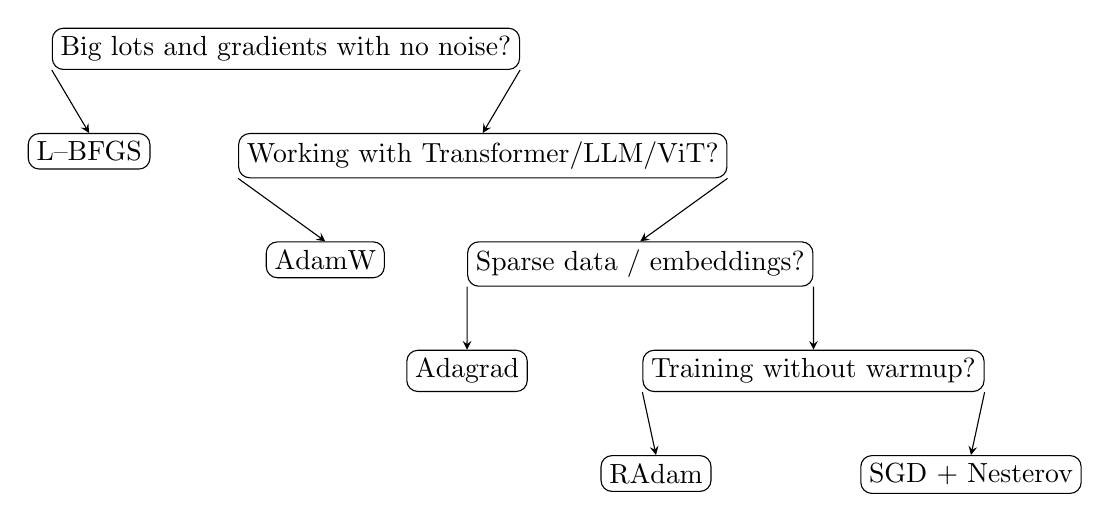
\begin{tikzpicture}[
  node distance=8mm,
  box/.style={rectangle, rounded corners, draw, align=left, inner sep=3pt},
  yes/.style={->,>=stealth},
]
\node[box] (q1) {Big lots and gradients with no noise?};
\node[box, below=of q1, xshift=-25mm] (lbgfs) {L\textendash BFGS};
\node[box, below=of q1, xshift=25mm] (q2) {Working with Transformer/LLM/ViT?};
\node[box, below=of q2, xshift=-20mm] (adamw) {AdamW};
\node[box, below=of q2, xshift=20mm] (q3) {Sparse data / embeddings?};
\node[box, below=of q3, xshift=-22mm] (adagrad) {Adagrad};
\node[box, below=of q3, xshift=22mm] (q4) {Training without warmup?};
\node[box, below=of q4, xshift=-20mm] (radam) {RAdam};
\node[box, below=of q4, xshift=20mm] (sgd) {SGD + Nesterov};

\draw[yes] (q1.south west) -- (lbgfs.north);
\draw[yes] (q1.south east) -- (q2.north);
\draw[yes] (q2.south west) -- (adamw.north);
\draw[yes] (q2.south east) -- (q3.north);
\draw[yes] (q3.south west) -- (adagrad.north);
\draw[yes] (q3.south east) -- (q4.north);
\draw[yes] (q4.south west) -- (radam.north);
\draw[yes] (q4.south east) -- (sgd.north);
\end{tikzpicture}
\end{frame}

% preâmbulo: \usepackage[most]{tcolorbox}

\begin{frame}{Areas of study}
\small
\begin{itemize}\itemsep0.25em
  \item \textbf{Optimization vs generalization:} \cite{keskar2016large} why does SGD often generalize better than AdamW in vision?
  \item \textbf{Sharpness \& flatness:} \cite{dinh2017sharp} Is flatness truly a reliable indicator of generalization in deep networks?
  \item \textbf{Scaling laws interplay:} \cite{kaplan2020scaling} how LR, schedule, and batch size co-vary optimally at trillion-token scale?
\end{itemize}
\end{frame}

\begin{frame}{Key takeaways}
\small
\begin{itemize}\itemsep0.3em
  \item Start simple: SGD+momentum (vision) or AdamW (transformers), warmup + cosine.
  \item Schedules matter as much as the optimizer; tune LR first, then weight decay/momentum.
  \item Consider SAM/Lookahead when generalization/stability is a pain point.
  \item Large batches: add LARS/LAMB trust ratios and longer warmup.
  \item For small/smooth problems, L-BFGS/Newton can be very effective.
\end{itemize}
\end{frame}

\section{References} 
\begin{frame}[allowframebreaks]
        \frametitle{Bibliography} 
        \bibliographystyle{ieeetr}
        \bibliography{assets/presentation_bib.bib}
\end{frame}


\backmatter
\end{document}
